\chapter{Proposta}

Este capítulo apresenta o método utilizado para a elaboração deste trabalho. Assim, para avaliar o impacto do uso do mecanismo de dicas personalizadas no ensino de conceitos básicos de programação, primeiramente será realizado a implementação do \foreign{iHint} utilizando o \foreign{framework} de desenvolvimento Laravel\footnote{\url{https://laravel.com/}}. Subsequente, será efetuado um estudo com os dados gerados nos experimentos presenciais para realizar a avaliação do sistema. A \cref{figura:visaometodo} ilustra cada etapa a ser realizada para o desenvolvimento da abordagem proposta.

\begin{figure}[h]
	\captionsetup{justification=centering}
	\includegraphics[width=\linewidth]{proposta/visaogeraldometodoproposto.png}
	\caption{Visão geral do método proposto.}
	\label{figura:visaometodo}
\end{figure}

\section{Implementação do \foreign{iHint}}

Esta seção, descreve o sistema de dicas a ser desenvolvido. O caso de uso da \cref{figura:sistemadicas} apresenta as funcionalidades do \foreign{iHint} que serão modeladas.

\begin{figure}[h]
	\centering
	\captionsetup{justification=centering}
	\includegraphics[width=.7\linewidth]{proposta/sistemadicas.png}
	\caption{Visão geral do sistema de dicas.}
	\label{figura:sistemadicas}
\end{figure}

\subsection{Gerenciar Usuário}

Quando um usuário desejar realizar o cadastro no sistema, ele poderá escolher entre a opção de aluno ou professor. O aluno, realiza exercícios disponíveis no banco de dados do sistema, preenche um diário não obrigatório para cada exercício, cria uma dica para cada exercício e consulta seu perfil com seus dados pessoais e um relatório de suas submissões de exercícios. O professor, além de realizar as mesmas atividades do aluno, também poderá criar salas com exercícios pré-definidos convidando alunos para fazer parte dela e submeter exercícios para o sistema. 

Primeiramente para o usuário se cadastrar no sistema, a primeira etapa é informar o nome, um e-mail e a senha para o cadastro. O sistema irá verificar se o e-mail do usuário está no formato "exemplo@exemplo.com", verificar se o e-mail já está registrado no banco de dados e realizar a comparação do valor do campo de senha com o do campo confirmar senha. Esta funcionalidade já foi implementada conforme a tela do sistema representada na \cref{figura:registrarusuario}.

\begin{figure}[]
	\captionsetup{justification=centering}
	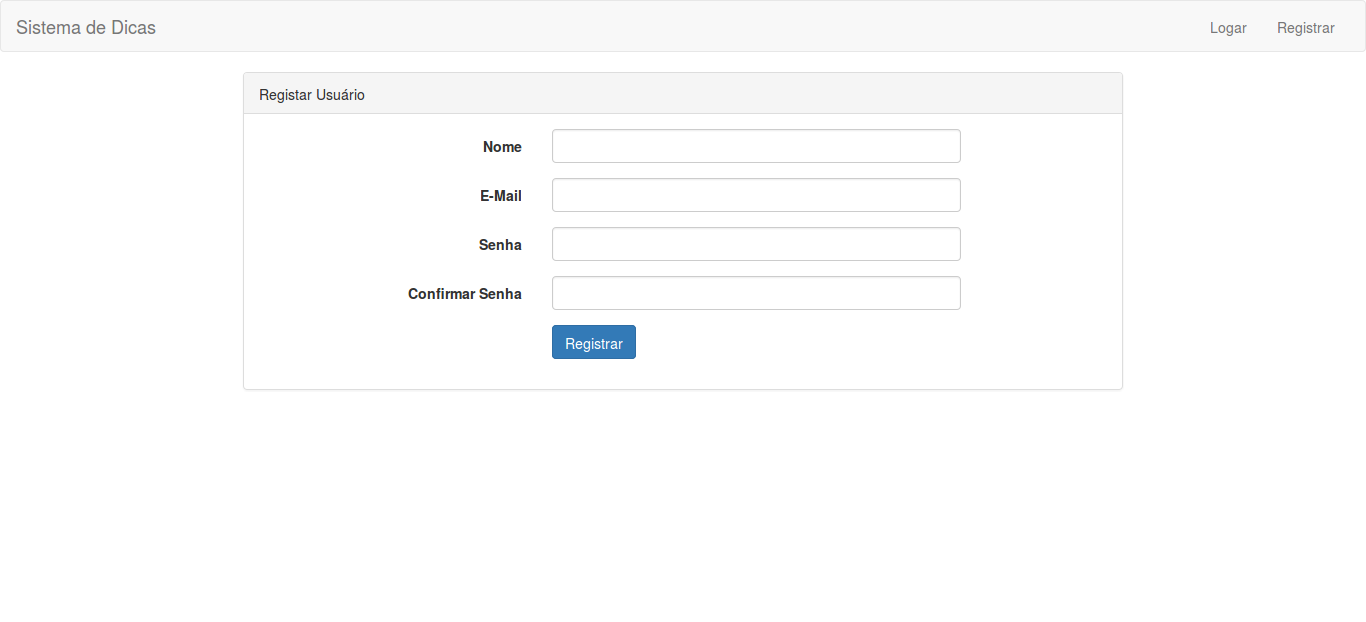
\includegraphics[width=\linewidth]{imagenssoftware/registrarusuario.png}
	\caption{Tela de regustro de usuário.}
	\label{figura:registrarusuario}
\end{figure}

Após o usuário estar cadastrado no sistema, ele poderá realizar o \foreign{login} através da tela representada na \cref{figura:logar} informando o e-mail e a senha.

\begin{figure}[]
	\captionsetup{justification=centering}
	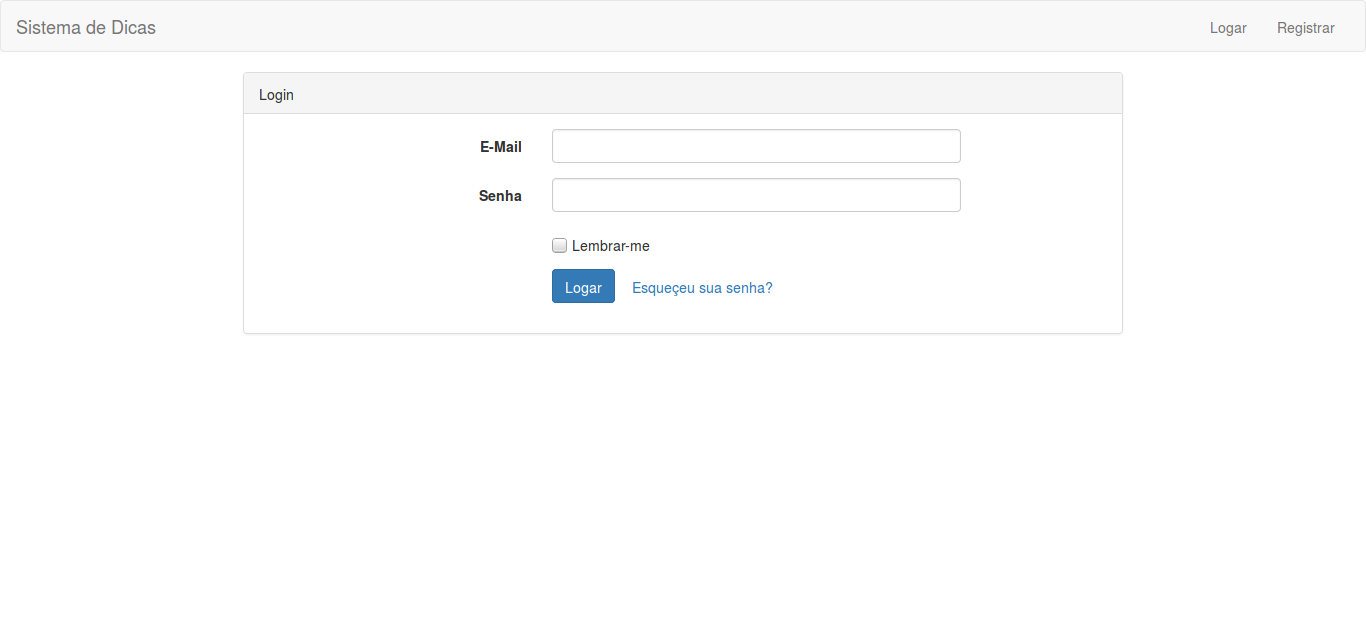
\includegraphics[width=\linewidth]{imagenssoftware/logar.png}
	\caption{Tela de login no sistema.}
	\label{figura:logar}
\end{figure}

Se o usuário estiver realizando o \foreign{login} pela primeira vez, ele terá que escolher se será um aluno ou professor e terá que preencher os campos apresentados nas \cref{figura:cadastroprofessor,figura:cadastroaluno}

\begin{figure}[]
	\centering
	\captionsetup{justification=centering}
	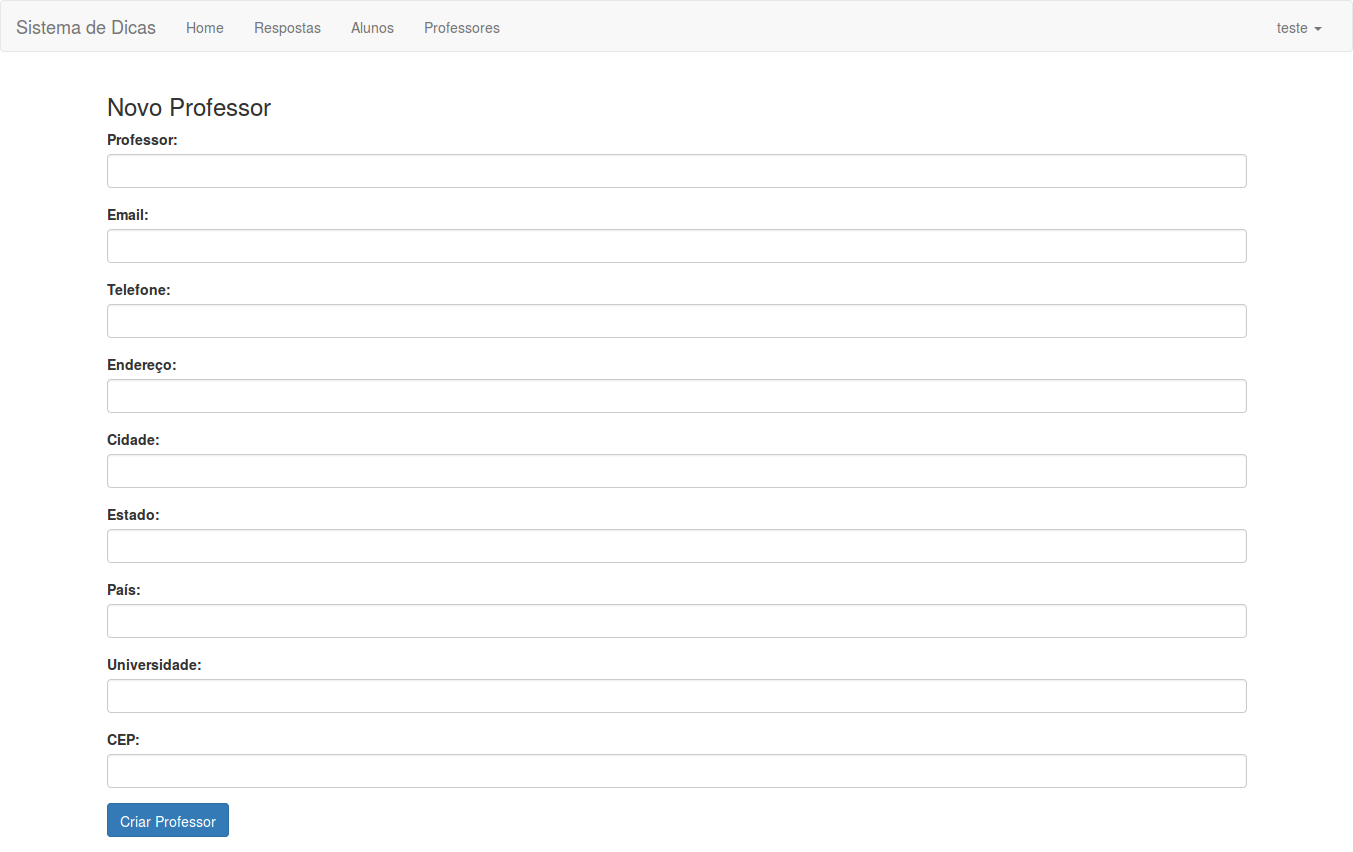
\includegraphics[width=.8\linewidth]{imagenssoftware/cadastroprofessor.png}
	\caption{Tela de cadastro de professor.}
	\label{figura:cadastroprofessor}
\end{figure}

\begin{figure}[]		
	\centering
	\captionsetup{justification=centering}
	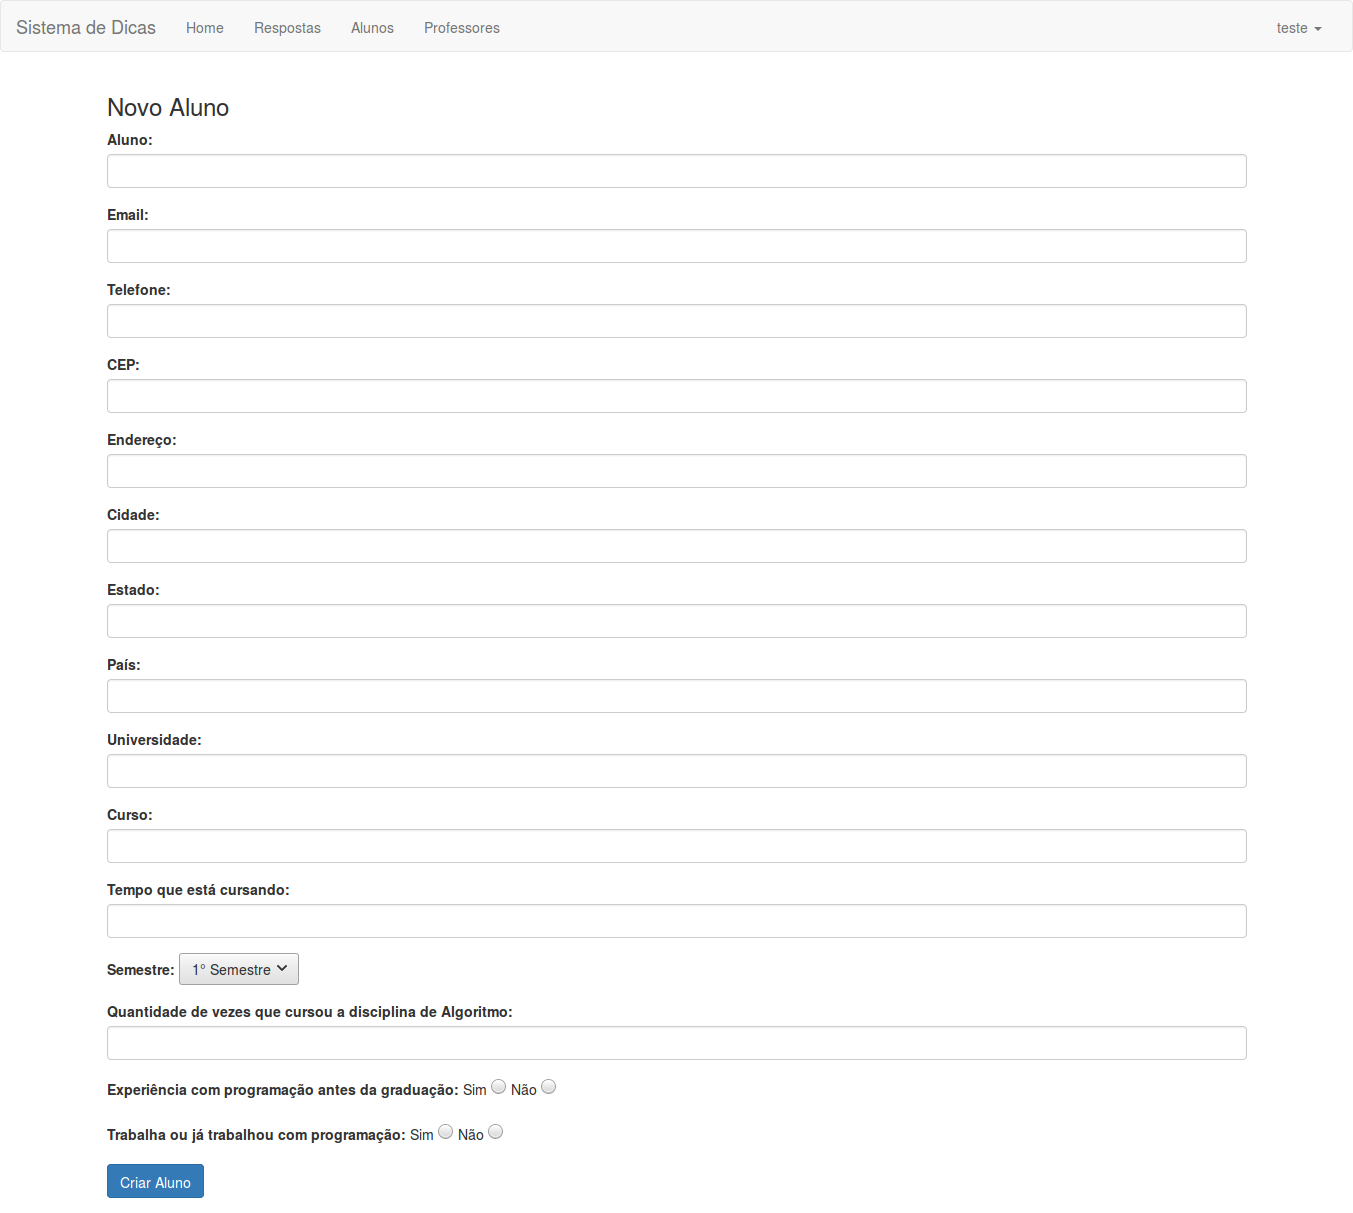
\includegraphics[width=.8\linewidth]{imagenssoftware/cadastroaluno.png}
	\caption{Tela de cadastro de aluno.}
	\label{figura:cadastroaluno}
\end{figure}

\frontmatter

\subsection{Gerenciar Exercício}

Essa funcionalidade do sistema só poderá ser acessada se o usuário for um professor. Sendo assim, o professor terá que cadastrar um enunciado, a linguagem de programação que o aluno deve utilizar para resolver o exercício, o nível (fácil, médio ou difícil), o tipo do exercício (condicional ou laço de repetição), e a resposta que poderá ser escrita em um campo ou um \foreign{upload} do arquivo com as respostas. Cada exercício cadastrado será agregado a uma lista de exercícios que o professor irá criar antes de cadastrar os exercícios.

\subsection{Lista de Exercício}

O professor poderá realizar o cadastro de uma lista de exercícios informando o nome da lista, os exercícios que deseja adicionar, o tempo máximo que um aluno deve realizar a lista. Os exercícios serão adicionados a partir da consulta no banco de dados de exercícios, para realizar a consulta o professor deverá informar o nível da dificuldade que deseja e o tipo do exercício (condicional ou laço de repetição). Desta forma, o sistema irá retornar uma lista com os exercícios que satisfazem a consulta, assim o professor poderá escolher os exercícios que deseja adicionar na lista.

\subsection{Gerenciar Turma}

O professor poderá realizar o cadastro de uma classe para adicionar seus alunos e passar as listas de exercícios e acompanhar o rendimento de cada aluno. Para cadastrar uma turma é necessário um nome da turma e um professor, com isso o professor poderá adicionar os alunos desejados ou gerar um código da sua turma através do sistema e disponibilizar para os alunos se cadastrarem.

\subsection{Realizar Exercício}

Após a conclusão do cadastro de usuário, o aluno ou professor terão acesso as funcionalidades específicas de cada tipo de usuário. Dessa forma, o usuário poderá resolver uma lista de exercícios estando vinculado a uma turma, assim ele poderá resolver a lista de exercícios que o professor responsável pela turma criou. Caso o usuário não faça parte de uma turma, ele terá que pesquisar por uma lista de exercícios informando qual assunto, estrutura de condição ou laço de repetição, ele deseja realizar. 

Depois que o usuário encontrar uma lista de exercícios, o sistema apresentará os exercícios à serem resolvidos na ordem em que foram adicionados na lista. Assim o usuário poderá trabalhar em sua solução e submeter ao sistema para correção utilizando a linguagem de programação escolhida pelo professor na criação da lista de exercícios, essa resolução poderá estar correta ou não. Se estiver correta, o sistema apresentará uma mensagem de parabenização e redirecionará o usuário para o próximo exercício. Caso a resolução estiver errada o sistema retornará qual o erro ocorrido na compilação, assim o usuário poderá realizar outras submissões até que consiga obter sucesso na resolução ou requisitar uma dica para o sistema para auxiliá-lo na construção da resposta. 

Cada submissão, tanto correta ou incorreta, é gravada no banco de dados na forma de \foreign{log}, sendo salvo os dados: a usuário que realizou o exercício, todas as submissões, os erros cometidos, o tempo demorado para obter sucesso no exercício, data e dicas utilizadas.

\subsubsection{Utilização das Dicas}

O usuário apenas poderá consultar uma dica caso o exercício enviado para validação não esteja correto e ele escolha a opção de disponibilização de dicas, assim ele terá direito a três dicas selecionadas aleatoriamente pelo mecanismo. O usuário irá escolher consultar uma das três dicas e após a consulta ele poderá realizar uma nova submissão do exercício.

\subsubsection{Boca (\textit{BOCA Online Contest Administrator})}

Para realizar a compilação dos exercícios no sistema de dicas, será utilizado funções do BOCA, um \foreign{software} livre\footnote{\url{https://github.com/cassiopc/boca/}} desenvolvido por \citeonline{de2004boca}, o BOCA é um sistema de entrega de exercícios, com autenticação, controle de tempo e disponibilização de resultados, tudo em tempo real. Toda a programação do sistema foi feita na linguagem PHP, e assim é portável para todo sistema onde tal linguagem esteja disponível. Para armazenamento dos dados e controle de concorrência é utilizado o banco de dados relacional \foreign{PostgreSQL}. 

O Boca funciona através do envio das resoluções realizada por usuários que enviam um arquivo-fonte para a validação do sistema, o resultado é retornado para o usuário o mais breve possível. No momento em que o usuário submete seu arquivo-fonte, ele poderá escolher a linguagem que o programou e para qual problema ele é destinado. Através do ambiente de janelas do navegador do BOCA, o usuário escolhe o arquivo do disco que deseja submeter e o envia para correção, o BOCA irá compilar esse arquivo-fonte e irá enviar um resultado para o usuário.

\subsection{Gerenciar Dica}

O cadastro de uma dica pode ser realizado quando o usuário submete um exercício para validação e obtêm êxito, assim o sistema apresentará uma tela perguntando se o usuário deseja contribuir com uma dica, caso aceite, o sistema irá redirecionar o usuário para a tela onde será realizado o cadastro da dica, onde ele irá descrever em um campo a dica que deseja compartilhar. Também será apresentada a solução do mesmo exercício de outro usuário para que seja escrito uma dica. 

\subsection{Gerenciar Diário}

No processo de execução de um exercício o usuário poderá preencher um diário relatando suas experiências, essa funcionalidade será apresentada aos usuários caso o professor deseja receber o preenchimento do diário dos exercícios da lista. 

Caso o professor pretende receber os diários dos exercícios da lista de sua turma, o usuário após cada submissão da resolução no sistema produzirá um diário que será informado os dados referentes a experiência de realizar o exercício. 

\subsection{Teste do sistema}

Após o desenvolvimento do sistema ser concluído, será necessário executar uma etapa de teste para encontrar possíveis erros no sistema. Para que essa etapa aconteça, será convocado um grupo de alunos da UTFPR do Curso de Bacharelado em Ciência da Computação de forma voluntária para utilizarem as funcionalidades do sistema, o estudo será realizado em um laboratório com a supervisão de um professor ou aluno. Os alunos deverão reportar os erros encontrados através de criação de \foreign{issues} no \foreign{GitHub} \footnote{\url{https://github.com/gustavoCorreiaGonzalez/aplicacao-tcc }}. Todos os erros serão corrigidos antes de realizar os estudos para avaliar o sistema.

\section{Estudo de Avaliação}

Esta seção apresentará o formato do estudo, descrevendo como serão realizados o teste do sistema, a criação do banco de exercícios, banco de dicas e como serão respondidas as questões de pesquisa.

\subsection{Banco de Exercícios}

Para que o estudo e a avaliação do sistema sejam possíveis, será necessário criar um banco de dados de exercícios a partir de exercícios selecionados para diferir dos exercícios realizados na matéria de Algoritmos oferecida pelo curso, a seleção terá a finalidade de prevenir que o voluntário do estudo de avaliação do sistema já tenha realizado o exercício. Os exercícios serão divididos em três grupos, o primeiro abordará conceitos básicos da linguagem de programação como entrada e saída de dados, declaração de variáveis e constantes, operações e funções matemáticas. O segundo grupo refere-se a estruturas condicionais e o terceiro grupo trata de estruturas de repetição.

\subsection{Banco de Dicas}

Para realizar o estudo UTFPR com os voluntários, será preciso que o sistema já tenha algumas dicas cadastradas no banco de dados. Deste modo, o banco de dicas será provido após a conclusão do banco de exercícios, assim será realizada uma convocação por formulário \foreign{online} aos estudantes da UTFPR do curso de Bacharelado em Ciência da Computação para se voluntariarem a utilizar o sistema de dicas por um determinado período em um dia que será estipulado no formulário. Os voluntários utilizaram o sistema de dicas em um ambiente controlado sendo esse um laboratório da UTFPR com um professor ou aluno monitorando as atividades e tirando as possíveis dúvidas dos participantes. 

\begin{figure}[]
	\centering
	\captionsetup{justification=centering}
	\includegraphics[width=.5\linewidth]{proposta/fluxoreflexao.png}
	\caption{Fluxos de reflexão para criação de dicas.}
	\label{figura:fluxoreflexao}
\end{figure}

\begin{figure}[]
	\centering
	\captionsetup{justification=centering}
	\includegraphics[width=.5\linewidth]{proposta/fluxocomparacao.png}
	\caption{Fluxos de comparação para criação de dicas.}
	\label{figura:fluxocomparacao}
\end{figure}

A criação das dicas ocorrerá conforme dois fluxos de execução, sendo eles: fluxo de reflexão representado pela \cref{figura:fluxoreflexao} e fluxo de comparação representado pela \cref{figura:fluxocomparacao}. Os dois fluxos são iniciados quando o usuário recebe uma lista de exercícios para ser realizada. No momento em que o usuário ter uma lista de exercícios o fluxo de reflexão começa. O sistema irá apresentar um exercício da lista para ser resolvido e o usuário poderá começar a realizar a solução, o aluno poderá requisitar ao sistema que necessita realizar uma consulta a algumas dicas. Deste modo, o sistema apresentará XXXX dicas para o aluno consultar e realizar sua solução.

Após a solução ser concluída, o usuário submete a solução para validação, o BOCO que irá executar a solução do exercício e verificar se está correta ou não. Caso a solução não estiver correta, o sistema redireciona para a etapa de realização de solução, nessa etapa o usuário poderá pedir uma dica para o sistema. Caso a solução estiver correta, o sistema irá redirecionar o usuário para a tela aonde ele criará a dica para o exercício e irá realizar o cadastro dela no banco de dicas.

Após o usuário gerar uma dica do exercício realizado, o sistema irá seguir o fluxo de comparação. Neste fluxo, o sistema irá procurar no banco de dados soluções de outros usuários do exercício realizado. O sistema irá apresentar ao usuário uma das piores e a uma das melhores soluções do exercício para que ele crie uma dica para melhorar as soluções. Para o sistema conseguir distinguir uma boa solução de outra ruim, cada solução será classificada tendo em conta os dados da execução do exercício e as métricas retiradas do código. Na execução do exercício será avaliado o tempo para a resolução correta do exercício, quantidade de dicas utilizadas e quantidades de tentativas erradas. No entanto, as métricas do código serão medidas através do número de linhas entre as tentativas, complexidade ciclomática e tamanho da solução. Com esses dados analisados, o sistema poderá realizar um \foreign{ranking} com as soluções e será considerado 25\% das primeiras posições como o grupo das melhores soluções e 25\% das últimas colocação como sendo o grupo das piores soluções. Assim, o sistema irá retornar para o aluno duas soluções que serão selecionadas de forma aleatória, sendo uma do grupo das melhores soluções e a outra do grupo das piores soluções.

A partir das soluções apresentadas ao aluno pelo sistema, ele poderá analisar e gerar uma dica para melhorar as soluções. Essas dicas de otimização serão cadastradas no banco de dados de dicas para auxiliar outros usuários na resolução do exercício.

\subsection{Avaliação do Sistema de Dicas}

\begin{figure}[]
	\centering
	\captionsetup{justification=centering}
	\includegraphics[width=.8\linewidth]{proposta/estudo.png}
	\caption{Visão geral da aplicação do estudo.}
	\label{figura:estudo}
\end{figure}

Nesta subseção será explicado as duas etapas que serão realizadas para responder as duas questões de pesquisa citadas abaixo.

\begin{itemize}
	\item \textbf{QP}\textsubscript{1}: 
	\textit{Existe impacto do uso do mecanismo de dicas para minimizar erros e melhorar soluções de exercícios?}
	\foreign
	\item \textbf{QP}\textsubscript{2}: 
	\textit{Quais dicas personalizadas ajudam mais os alunos?}
\end{itemize}

Enquanto \textbf{QP}\textsubscript{1} tem como objetivo investigar se o mecanismo de dicas irá ajudar os alunos a obterem melhores resultados na resolução de exercícios de programação. \textbf{QP}\textsubscript{2} avaliará qual tipo de dica é melhor, podendo ser aleatorizadas em função do tipo do exercício, geradas a partir de erros cometidos em exercícios passados e sem dicas. Levando em consideração a fonte da dica gerada, podendo ser por alunos iniciantes, alunos experientes ou professores.

A primeira etapa consiste em aplicar um estudo controlado na UTFPR para gerar os dados de \foreign{log} de submissões das listas de exercícios. Dessa forma, após a geração dos dados de \foreign{log} a segunda etapa será inicializada. A segunda etapa apresenta as análises que serão feitas para responder as questões de pesquisa.

\begin{table}[]
	\centering
	\captionsetup{justification=centering}
	\caption{Formulário para aquisição de voluntários.}
	\label{tabela:formulário}
	\begin{tabular}{l}
		\hline
		Perguntas                        \\ \hline
		Nome?                            \\
		Idade?                           \\
		Telefone?                        \\
		Email?                           \\
		Curso?                           \\
		Tempo que está cursando o curso? \\
		Qual semestre você está?         \\ 
		Quantidade de vezes que cursou a disciplina de Algoritmos?  \\ 
		Teve experiência com programação antes da graduação? \\
		Trabalha ou já trabalhou com programação? \\ \hline
	\end{tabular}
\end{table}

A Figura \ref{figura:estudo} representa a primeira etapa da avaliação do sistema, onde será necessário a colaboração de voluntários do curso de Bacharelado em Ciência da Computação para o experimento presencial que será realizado na UTFPR, para isso será criado um formulário no \foreign{Google Forms} representado na Tabela \ref{tabela:formulário} e disponibilizado \foreign{online} para os alunos do curso.

Os voluntários serão divididos em três grupos distintos de acordo com o nível de conhecimento em programação, o nível de cada voluntário será estimado de acordo com o tempo que está na graduação e o semestre que se encontra. Os três grupos irão realizar os mesmos exercícios mas utilizaram funcionalidades diferentes do sistema,  

\begin{itemize}
	\item \textbf{Grupo 1}: Utilizará o mecanismo de dicas que prove dicas de acordo com o exercício que o aluno está realizando.
	
	\item \textbf{Grupo 2}: Utilizará o mecanismo de dicas personalizado que disponibiliza dicas de acordo com o exercício e o erro cometido na submissão.

	\item \textbf{Grupo 3}: Utilizará o sistema sem o mecanismo de dicas.
\end{itemize}

Toda submissão realizada pelos três grupos de voluntários será gravada no \foreign{log} de submissões, sendo salvo os dados: a usuário que realizou o exercício, todas as submissões, os erros cometidos, o tempo demorado para obter sucesso no exercício. Após todos os voluntários tiverem finalizados todos os exercícios da lista, o estudo presencial será finalizado com a aplicação de um questionário representado na Tabela \ref{tabela:questionárioestudo} para avaliar a usabilidade do sistema e a experiência da utilização de um sistema \foreign{web} para solucionar exercícios de programação.

\begin{table}[]
	\centering
	\captionsetup{justification=centering}
	\caption{Questionário do estudo presencial.}
	\label{tabela:questionárioestudo}
	\begin{tabular}{l}
		\hline
		Perguntas                        \\ \hline
		pergunta1?                            \\
		pergunta2?                           \\
		pergunta3?                        \\
		pergunta4?                           \\
		pergunta5?                           \\
		pergunta6? \\
		pergunta7?                        \\ \hline
	\end{tabular}
\end{table}

A segunda etapa da avaliação do sistema responderá as duas questões de pesquisa, será analisado os dados do \foreign{log} de submissões realizados na primeira etapa. A primeira questão de pesquisa será respondida a partir da avaliação do desempenho dos grupos que utilizaram o sistema no estudo controlado. Será realizada uma comparação estatística para avaliar as hipóteses descritas abaixo. 

\begin{itemize}
	\item \textbf{Hipótese 1}: O grupo 1 desenvolverá soluções melhores com a utilização dos mecanismos de dicas em relação as soluções do grupo 3.
	\item \textbf{Hipótese 2}: O grupo 2 desenvolverá soluções melhores com a utilização dos mecanismos de dicas personalizadas em relação as soluções do grupo 3.	
	\item \textbf{Hipótese 3}: O grupo 1 desenvolverá soluções melhores com a utilização dos mecanismos de dicas em relação as soluções do grupo 2.	
	\item \textbf{Hipótese 4}: O grupo 2 desenvolverá soluções melhores com a utilização dos mecanismos de dicas personalizadas em relação as soluções do grupo 1.
\end{itemize}

A segunda questão será respondida com a análise estatística da comparação do desempenho do grupo 1 de voluntário com o grupo 2, será verificado se as dicas dos voluntários mais experientes possuíram melhor avaliação em relação as dicas dos voluntários menos experientes.